\chapter{Proposal}
\label{ch.proposal}

A proposta desta dissertação é composta por duas contribuições principais.
A primeira contribuição será o porte do modulo de comunicação entre clusters
descrito na Seção \ref{sec.inter-cluster-communication} para o processador manycore MPPA.
A segunda contribuição será o projeto e implementação de serviços de comunicação de
um sistema operacional mestre-escravo encima desse módulo de comunicação.

\section{Inter-Cluster Communication Module}

    Idealmente, a implementação da HAL não deveria utilizar nenhuma outra camada
	de software para conversar com o hardware.
	Porém, a implementação da HAL no MPPA utiliza-se de camadas indispensáveis
	da pilha de software disponibilizada pela Kalray.
	Para substituí-las seria necessário um grande esforço, fugindo da proposta
	deste trabalho e do escopo do doutorado do Pedro H. Penna.
	Os principais motivos para essa decisão foram devido a documentação pobre
	e a impossibilidade de executar código em modo kernel livremente.
	
	\begin{figure}[t]
		\centering
		\caption{Software Stack of the \mppa.}

		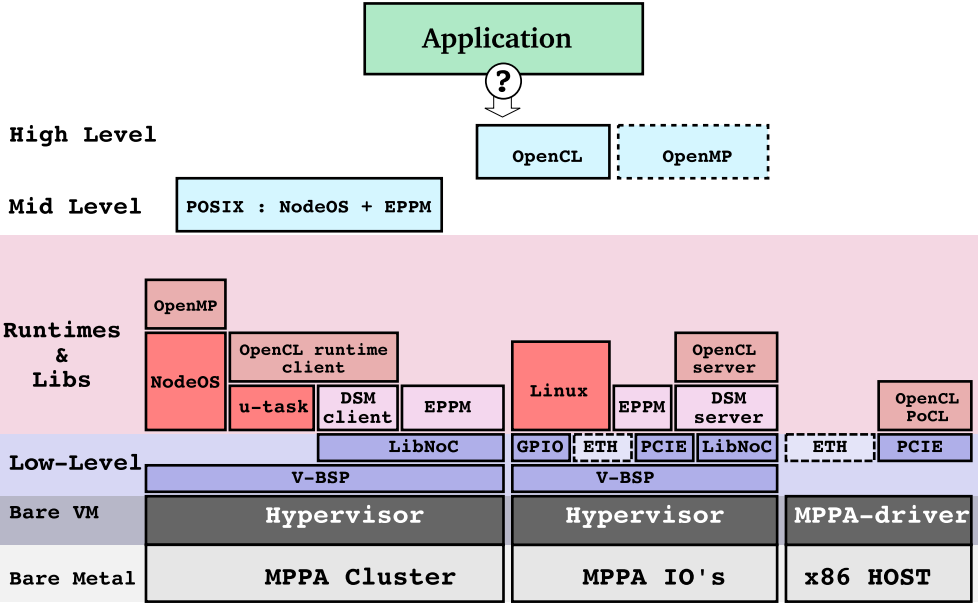
\includegraphics[width=.7\textwidth]{images/software-stack.png}

		Source: \mppa Processor Documentation.

		\label{fig.conpt_sync}
	\end{figure}

	A Figure X mostra a pilha de software presente para o MPPA.
	A partir dela, serão utilizados apenas o hypervisor e a biblioteca vbsp.
	O hypervisor é utilizado para virtualizar o hardware separando-o em partes lógicas,
	e.g., virtualização do núcleo, da interface cnoc e da interface dnoc.
	Ele também exporta rotinas para gerenciar, configurar e permitir acesso aos recursos virtuais.
	A biblioteca vbsp, por sua vez, prove primitivas para configuração de interrupções.

	O módulo de comunicação entre clusters utilizará interfaces da própria HAL
	e as virtualizações das interfaces cnoc e dnoc diretamente.
	As interfaces virtuais exportam chamadas assíncronas para adquirir permissão de leitura e escrita
	direta de registradores que configuram o hardware para determinada tarefa.
	Por exemplo, a configuração da DMA para envio assíncrono é abstraido por
	micro-threads que são configuradas através de estruturas globais providas pelo hypervisor.

    \begin{table}[t]
        \caption{Cluster Identification.}

        \begin{tabular}{|l|l|l|}
            \hline
                        & Physical ID & Logical ID \\ \hline
            \ccluster   & 0-15        & 0-15       \\ \hline
            \iocluster0 & 128-131     & 16-19      \\ \hline
            \iocluster1 & 192-195     & 20-23      \\ \hline
        \end{tabular}

        \label{tab.cluster-id}
    \end{table}

    Os clusters possuem dois identificadores, um físico e outro lógico.
    Os identificadores físicos são os números em hardware que identica-los
    durante o processo de roteamento dos dados através da \noc.
    Os identificadores lógicos são números associados aos identificadores
    lógicos para que seja possível identificar os clusters fora da \hal.
    Os identificadores lógicos servem principalmente para desassociar
    a identificação de um cluster da arquitetura no qual a \hal está implementada,
    como ilustrado na Tabela X.

    \begin{table}[]
        \caption{Partitions of \noc resources by abstraction.}

        \begin{tabular}{l|l|l|l|l|}
            \cline{2-5}
                                           & \multicolumn{2}{c|}{\cnoc} & \multicolumn{2}{c|}{\dnoc} \\ \cline{2-5} 
                                           & RX Slot & TX Channel & RX Slot & TX Channel \\ \hline
            \multicolumn{1}{|l|}{\mailbox} & 0-23    & 0          & 0-23    & 1-3        \\ \hline
            \multicolumn{1}{|l|}{\portal}  & 24-47   & 1-2        & 24-47   & 4-7        \\ \hline
            \multicolumn{1}{|l|}{\sync}    & 48-71   & 3          & -       & -          \\ \hline
        \end{tabular}

        \label{tab.cluster-id}
    \end{table}

    Para realizar a comunicação entre dois cluster é necessário saber
    que o emissor conheça qual o recurso que o receptor vai utilizar.
    Por este motivo, o intervalo de slot de recebimento da cnoc e dnoc
    são repartidos por abstração, como pode ser visto na Tabela A.
    Dentro de uma partição, um slot é associado a cada identificador lógico dos cluster.
    Por outro lado, os emissores utilizam canais de envio que precisam
    ser reservados durante toda a operação, para isso, a Tabela A também mostra
    a partição dos canais para cada abstração.

    \subsection{Sync}

    % \todo[inline]{
    %     Quais são as funções?
    %     Como pretendes implementá-las?
    %     Quais são os recursos (API ou hardware) do MPPA que serão
    %     explorados para implementar essa interface?
    % }

\begin{figure}[t]
\begin{lstlisting}[
    caption=HAL Sync Interface for Receiver Cluster,
    label=cod:sync-receiver,
]
    /* @brief Allocates and configures the receiving side of
     *        the synchronization point.                     */
    int sync_create(const int *nodes, int nnodes, int type);

    /* @brief Releases and cleans receiver buffer. */
    int sync_unlink(int syncid);

    /* @brief Wait signal on a specific synchronization point. */
    int sync_wait(int syncid);
\end{lstlisting}
\end{figure}

\begin{figure}[t]
\begin{lstlisting}[
    caption=HAL Sync Interface for Sender Cluster,
    label=cod:sync-sender,
]
    /*  @brief Allocates and configures the sending side of
     *  the synchronization point.                          */
    int sync_open(void);

    /* @brief Releases the sender resources on a specific DMA channel. */
    int sync_close(int syncid);

    /* @brief Send signal on a specific synchronization point. */
    int sync_signal(int syncid, const int *nodes, int nnodes, int type);
\end{lstlisting}
\end{figure}

        A abstração \sync pode ser decomposta em dois conjuntos de funções, um para
        os clusters que irão receber sinais e outro para os que irão enviar.
        Cada conjunto aloca tipos diferentes de recursos.
        Espeficicamente, o receptor deverá alocar um slot de recebimento da cnoc
        e o emissor alocará um canal de emissão da cnoc.
        Devido a isso, poderão ser criados 24 pontos de sincronização (\texttt{sync\_create()})
        e aberto apenar 1 por (\texttt{sync\_open()}) cluster.

        As funções implementam dois tipos diferentes dependendo de quem
        deve ser o mestre da operação de sincronização.
        Isto é, toda operação de sincronização é separada em um cluster mestre
        e um ou mais clusters escravos, definidas pelas constantes
        \texttt{ONE\_TO\_ALL} e \texttt{ALL\_TO\_ONE}.
        O mestre sempre assume o papel "ONE" e os escravos o papel "ALL".
        As subseções abaixo descreveram o comportamento e detalhes de implementação
        de cada um dos tipos de sincronização.

            \subsubsection*{\texttt{ONE\_TO\_ALL} Synchronization Type}

                Os clusters escravos envolvidos neste tipo de sincronização esperam
                um sinal enviado do mestre.
                Para isso, cada escravo executará a função \texttt{sync\_create()}
                alocando o recurso associado ao identificador lógico do mestre.
                Após alocar e configurar o recurso, o cluster pode continuar
                executando sem se preocupar se o sinal foi recebido.
                Quando chegar a hora de realizar a sincronização, basta o escravo
                escutar a função \texttt{sync\_wait()}.
                Ao receber o sinal, o sync autoreconfigurará o recurso e liberará o cluster,
                caso ele esteja esperando.

                O mestre, por sua vez, deverá executar as funções complementares.
                Isto é, primeiramente, o mestre alocará um recurso de envio
                ao chamar a função \texttt{sync\_open()}.
                Após isso, ele deverá informar o conjunto de clusters que
                receberão o sinal para o seu identificador lógico.
                Por fim, ambos podem chamar as funções de liberação dos recursos
                de sincronização, \texttt{sync\_unlink()} para o escravo e
                \texttt{sync\_close()} para o mestre.

            \subsubsection*{\texttt{ALL\_TO\_ONE} Synchronization Type}

                Analogamente ao tipo anterior, apenas os papeis se invertem.
                O mestre deverá executar as funções de criação, configuração dos
                recursos e espera dos inúmeros sinais.
                O recurso alocado pelo mestre deverá ser o recurso associado ao
                seu próprio identificador lógico.
                Por outro lado, os escravos executarão as funções de abertura
                e envio de um sinal para o indentificador lógico do mestre.

    \subsection{Mailbox}

    % \todo[inline]{
    %     Quais são as funções?
    %     Como pretendes implementá-las?
    %     Quais são os recursos (API ou hardware) do MPPA que serão
    %     explorados para implementar essa interface?
    % }

\begin{figure}[t]
\begin{lstlisting}[
    caption=HAL Mailbox Interface for Receiver Cluster,
    label=cod:mailbox-receiver,
]
	/* @brief Creates a mailbox. */
	int mailbox_create(int nodenum);

	/* @brief Destroys a mailbox. */
	int mailbox_unlink(int mbxid);

    /* @brief Reads data from a mailbox. */
	ssize_t mailbox_read(int mbxid, void * buffer, size_t size);
\end{lstlisting}
\end{figure}

\begin{figure}[t]
\begin{lstlisting}[
    caption=HAL Mailbox Interface for Sender Cluster,
    label=cod:mailbox-sender,
]
    /* @brief Opens a mailbox. */
	int mailbox_open(int nodenum);

	/* @brief Closes a mailbox. */
	int mailbox_close(int mbxid);

	/* @brief Writes data to a mailbox. */
	ssize_t mailbox_write(int mbxid, const void * buffer, size_t size);
\end{lstlisting}
\end{figure}

        A abstração Mailbox é mais complexa que a abstração anterior utilizando
        tanto recursos da dnoc como da cnoc.
        Ao executar a função \texttt{mailbox\_create()}, o receptor utilizará
        apenas um slot de recebimento da dnoc alocando estaticamente uma
        quantidade suficiente para receber 24 mensagens dentro do espaço
        de memória do kernel.
        As mensagens são compostas por cabeçalho identificando o emissor
        e um corpo contendo a mensagem útil.
        Ao consumir uma mensagem (\texttt{mailbox\_read()}), o receptor copiará
        a mensagem para o buffer do usuário e enviará um sinal para o emissor
        informando-o que ele poderá enviar outra mensagem.
        Caso não exista nenhuma mensagem no buffer, o receptor é bloqueado
        até receber uma mensagem.

        Do outro lado, o emissor alocará um slot de recebimento de sinais
        (\texttt{mailbox\_open()} antes de enviar de enviar sua primeira mensagem ao receptor.
        Se o emissor tentar enviar uma mensagem antes do receptor ter consumido
        a mensagem anterior, o emissor ficará bloqueado esperando a notificação
        do emissor.
        Deste modo, o controle de fluxo é garantido e o emissor não
        sobreescreverá mensagens não-lidas pelo receptor.
        O envio da mensagem será sempre executado asincronamente porque
        sempre será necessário realizar a cópia da mensagem para um
        buffer do kernel que contenha o cabeçalho.
        Assim, o emissor nunca ficará bloqueado esperando a mensagem ser enviada.

        Nesta configuração, a quantidade de criações (\texttt{mailbox\_create()}) de
        mailbox dentro de um cluster é limitada a 1 por causa do canal de envio da cnoc.
        Por outro lado, a quantidade de aberturas (\texttt{mailbox\_open()}) é 4 por
        causa da limitação de canais de envio da dnoc disponíveis.

    \subsection{Portal}

    % \todo[inline]{
    %     Quais são as funções?
    %     Como pretendes implementá-las?
    %     Quais são os recursos (API ou hardware) do MPPA que serão explorados
    %     para implementar essa interface?
    % }

\begin{figure}[t]
\begin{lstlisting}[
    caption=HAL Portal Interface for Receiver Cluster,
    label=cod:portal-receiver,
]
	/* @brief Creates a portal. */
    int portal_create(int local);

	/* @brief Destroys a portal. */
    int portal_unlink(int portalid);

    /* @brief Allow sender to transfer data. */
    int portal_allow(int portalid, int remote);

    /* @brief Reads data asynchronously from a portal. */
    ssize_t portal_read(int portalid, void * buffer, size_t size);

    /* @brief Waits for an asynchronous operation on a
     *        portal to complete.                      */
    int portal_wait(int portalid);
\end{lstlisting}
\end{figure}

\begin{figure}[t]
\begin{lstlisting}[
    caption=HAL Portal Interface for Sender Cluster,
    label=cod:portal-sender,
]
    /* @brief Opens a portal. */
    int portal_open(int remote);

	/* @brief Closes a portal. */
    int portal_close(int portalid);

	/* @brief Writes data to a portal. */
    ssize_t portal_write(int portalid, const void * buffer, size_t size);

    /* @brief Writes data asynchronously to a portal. */
    int portal_awrite(int portalid, const void * buffer, size_t size);
    
    /* @brief Waits for an asynchronous operation on a
     *        portal to complete.                      */
    int portal_wait(int portalid);
\end{lstlisting}
\end{figure}

        A abstração \portal segue analogamente as ideias implementadas
        no \mailbox com a diferença da opção de escrever de forma
        síncrona ou assíncrona.
        O total de operações de recebimento de dados (\texttt{portal\_create()})
        é limitada a 2 por causa da quantidade de canais de envio de sinais disponiveis.
        Por outro lado, é possível realizar até 4 operações de envio (\texttt{portal\_open()})
        simultaneamente porque existem 4 canais de envio de dados disponíveis para o \portal.

        A função \texttt{portal\_open()} inicia a operação de envio de dados.
        Nele será alocado um canal de envio de dados associado uma micro-thread.
        Também será alocado um slot de recebimento de sinal para receber o sinal que
        liberará o envio de dados ao receptor.
        A operação de envio pode ser síncrona (\texttt{portal\_write()}) ou assíncrona (\texttt{portal\_awrite()}).
        Em uma operação assíncrona, o cluster não poderá modificar ou liberar o buffer até 
        que a operação seja completada.
        Para garantir que poderá utilizar o buffer o cluster chamar a função \texttt{portal\_wait()} .

        Para receber dados de outro cluster, o receptor alocará um slot de recebimento da dnoc
        e um canal de envio da cnoc através da função \texttt{portal\_create()}.
        Após configurar os recursos (\texttt{portal\_read()}), o receptor poderá
        notificar um emissor (\texttt{portal\_allow()}, habilitando-o a transferir dados. 
        Por este motivo, a operação de leitura é sempre realizada de forma assíncrona.
        Após receber a quantidade de dados configurada, o receptor poderá utilizar o buffer de forma segura.

    \section{Communication Services}

    % \todo[inline]{
    %     Quais são os serviços?
    %     Como pretendes implementá-los?
    %     Quais são os recursos (API ou hardware) do MPPA que serão explorados
    %     para implementar esses serviços?
    % }
